% ============================================================
%  Figure 2 — Motivation: Closed-Set CP vs. Embedding-Space CP
%  Standalone TikZ → compile with: pdflatex fig_motivation.tex
% ============================================================
\documentclass[border=6pt]{standalone}
\usepackage{tikz}
\usetikzlibrary{arrows.meta, positioning, decorations.pathreplacing,
                 calc, backgrounds}
\usepackage{amsmath,amssymb}
\usepackage{pifont}
\usepackage{xcolor}

\definecolor{cBlue}{HTML}{4C72B0}
\definecolor{cOrange}{HTML}{E8853A}
\definecolor{cGreen}{HTML}{55A868}
\definecolor{cRed}{HTML}{C44E52}
\definecolor{cPurple}{HTML}{8172B2}
\definecolor{cGray}{HTML}{999999}
\definecolor{cLightGray}{HTML}{F0F0F0}

\begin{document}
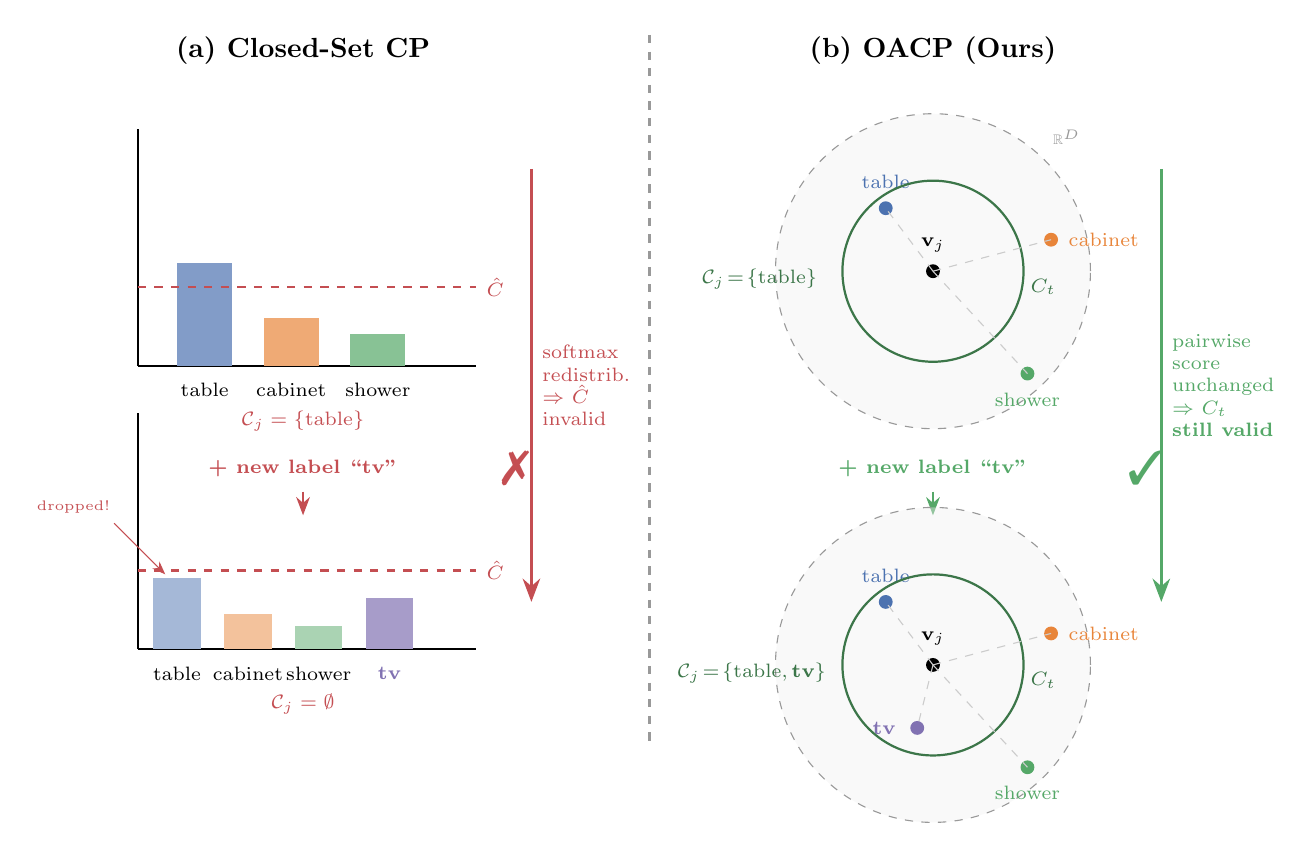
\begin{tikzpicture}[
    >=Stealth,
    font=\small,
]

% ================================================================
%  LEFT PANEL: Closed-Set Conformal Prediction
% ================================================================
\begin{scope}[shift={(0,0)}]

\node[font=\normalsize\bfseries] at (2.6, 4.0)
    {(a) Closed-Set CP};

% ── Top bar chart: K=3 classes ──
\draw[thick] (0.5, 0) -- (0.5, 3.0);
\draw[thick] (0.5, 0) -- (4.8, 0);

\fill[cBlue!70]   (1.0, 0) rectangle (1.7, 1.3);
\fill[cOrange!70] (2.1, 0) rectangle (2.8, 0.6);
\fill[cGreen!70]  (3.2, 0) rectangle (3.9, 0.4);

\node[font=\scriptsize, anchor=north] at (1.35, -0.1) {table};
\node[font=\scriptsize, anchor=north] at (2.45, -0.1) {cabinet};
\node[font=\scriptsize, anchor=north] at (3.55, -0.1) {shower};

% Threshold line
\draw[thick, dashed, cRed] (0.5, 1.0) -- (4.8, 1.0)
    node[right, font=\scriptsize, text=cRed] {$\hat{C}$};

% Prediction set
\node[font=\scriptsize, text=cRed] at (2.6, -0.7)
    {$\mathcal{C}_j = \{\text{table}\}$};

% ── Transition arrow ──
\node[font=\scriptsize\bfseries, text=cRed] at (2.6, -1.3) {+ new label ``tv''};
\draw[->, thick, cRed] (2.6, -1.6) -- (2.6, -1.9);

% ── Bottom bar chart: K+1 classes (redistributed!) ──
\begin{scope}[shift={(0, -3.6)}]
\draw[thick] (0.5, 0) -- (0.5, 3.0);
\draw[thick] (0.5, 0) -- (4.8, 0);

\fill[cBlue!50]    (0.7, 0) rectangle (1.3, 0.9);
\fill[cOrange!50]  (1.6, 0) rectangle (2.2, 0.45);
\fill[cGreen!50]   (2.5, 0) rectangle (3.1, 0.3);
\fill[cPurple!70]  (3.4, 0) rectangle (4.0, 0.65);

\node[font=\scriptsize, anchor=north] at (1.0, -0.1) {table};
\node[font=\scriptsize, anchor=north] at (1.9, -0.1) {cabinet};
\node[font=\scriptsize, anchor=north] at (2.8, -0.1) {shower};
\node[font=\scriptsize, anchor=north, text=cPurple] at (3.7, -0.1) {\textbf{tv}};

\draw[thick, dashed, cRed] (0.5, 1.0) -- (4.8, 1.0)
    node[right, font=\scriptsize, text=cRed] {$\hat{C}$};

% Arrow: table dropped below threshold
\draw[->, thin, cRed] (0.2, 1.6) -- (0.85, 0.95)
    node[pos=0, above left, font=\tiny, text=cRed, xshift=2pt] {dropped!};

\node[font=\scriptsize, text=cRed] at (2.6, -0.7)
    {$\mathcal{C}_j = \emptyset$};
\end{scope}

% Cross mark
\node[font=\LARGE, text=cRed] at (5.3, -1.3) {\ding{55}};

% Right-side annotation
\draw[very thick, cRed, ->] (5.5, 2.5) -- (5.5, -3.0)
    node[midway, right, font=\scriptsize, text=cRed, align=left]
    {softmax\\redistrib.\\$\Rightarrow$ $\hat{C}$\\invalid};

\end{scope}

% ================================================================
%  Divider
% ================================================================
\draw[thick, cGray, dashed] (7.0, 4.2) -- (7.0, -4.8);

% ================================================================
%  RIGHT PANEL: Embedding-Space CP (Ours)
% ================================================================
\begin{scope}[shift={(8.2, 0)}]

\node[font=\normalsize\bfseries] at (2.4, 4.0)
    {(b) OACP (Ours)};

% ── Top: 2D embedding space, K=3 ──
\begin{scope}[shift={(2.4, 1.2)}]

% Outer boundary (embedding space)
\fill[cLightGray, opacity=0.4] (0,0) circle (2.0);
\draw[cGray, dashed, thin] (0,0) circle (2.0);
\node[font=\tiny, text=cGray] at (1.7, 1.7) {$\mathbb{R}^D$};

% Visual feature (cell j)
\fill[black] (0, 0) circle (2.5pt);
\node[font=\scriptsize, anchor=south] at (0, 0.12) {$\mathbf{v}_j$};

% Text embeddings — placed with more space
\fill[cBlue]   (-0.6, 0.8) circle (2.5pt);
\node[font=\scriptsize, text=cBlue, anchor=south] at (-0.6, 0.92) {table};

\fill[cOrange] (1.5, 0.4) circle (2.5pt);
\node[font=\scriptsize, text=cOrange, anchor=west] at (1.6, 0.4) {cabinet};

\fill[cGreen]  (1.2, -1.3) circle (2.5pt);
\node[font=\scriptsize, text=cGreen, anchor=north] at (1.2, -1.42) {shower};

% Conformal radius (smaller!)
\draw[thick, cGreen!70!black] (0,0) circle (1.15);
\node[font=\scriptsize, text=cGreen!70!black] at (1.4, -0.2) {$C_t$};

% Dashed distance lines (all labels to v_j)
\draw[thin, cGray!50, dashed] (0,0) -- (-0.6, 0.8);
\draw[thin, cGray!50, dashed] (0,0) -- (1.5, 0.4);
\draw[thin, cGray!50, dashed] (0,0) -- (1.2, -1.3);

% Prediction set label
\node[font=\scriptsize, text=cGreen!70!black] at (-2.2, -0.1)
    {$\mathcal{C}_j\!=\!\{\text{table}\}$};

\end{scope}

% ── Transition arrow ──
\node[font=\scriptsize\bfseries, text=cGreen] at (2.4, -1.3) {+ new label ``tv''};
\draw[->, thick, cGreen] (2.4, -1.6) -- (2.4, -1.9);

% ── Bottom: K+1, same embedding space ──
\begin{scope}[shift={(2.4, -3.8)}]

\fill[cLightGray, opacity=0.4] (0,0) circle (2.0);
\draw[cGray, dashed, thin] (0,0) circle (2.0);

\fill[black] (0, 0) circle (2.5pt);
\node[font=\scriptsize, anchor=south] at (0, 0.12) {$\mathbf{v}_j$};

% Same positions — unchanged!
\fill[cBlue]   (-0.6, 0.8) circle (2.5pt);
\node[font=\scriptsize, text=cBlue, anchor=south] at (-0.6, 0.92) {table};

\fill[cOrange] (1.5, 0.4) circle (2.5pt);
\node[font=\scriptsize, text=cOrange, anchor=west] at (1.6, 0.4) {cabinet};

\fill[cGreen]  (1.2, -1.3) circle (2.5pt);
\node[font=\scriptsize, text=cGreen, anchor=north] at (1.2, -1.42) {shower};

% NEW label
\fill[cPurple] (-0.2, -0.8) circle (2.5pt);
\node[font=\scriptsize\bfseries, text=cPurple, anchor=east] at (-0.35, -0.8) {tv};

% Same conformal radius!
\draw[thick, cGreen!70!black] (0,0) circle (1.15);
\node[font=\scriptsize, text=cGreen!70!black] at (1.4, -0.2) {$C_t$};

% Dashed distance lines (all labels to v_j)
\draw[thin, cGray!50, dashed] (0,0) -- (-0.6, 0.8);
\draw[thin, cGray!50, dashed] (0,0) -- (1.5, 0.4);
\draw[thin, cGray!50, dashed] (0,0) -- (1.2, -1.3);
\draw[thin, cGray!50, dashed] (0,0) -- (-0.2, -0.8);

% Updated prediction set
\node[font=\scriptsize, text=cGreen!70!black] at (-2.3, -0.1)
    {$\mathcal{C}_j\!=\!\{\text{table},\textbf{tv}\}$};

\end{scope}

% Check mark
\node[font=\LARGE, text=cGreen] at (5.1, -1.3) {\ding{51}};

% Right-side annotation
\draw[very thick, cGreen, ->] (5.3, 2.5) -- (5.3, -3.0)
    node[midway, right, font=\scriptsize, text=cGreen, align=left]
    {pairwise\\score\\unchanged\\$\Rightarrow$ $C_t$\\\textbf{still valid}};

\end{scope}

\end{tikzpicture}
\end{document}
